\documentclass[a4paper]{report} 
%% in alternativa,\documentclass[a4paper]{book}

%% importazione di pacchetti utili
\usepackage[italian]{babel}
\usepackage{latexsym}
\usepackage{amssymb}
\usepackage{amsmath}
\usepackage{amsfonts}
\usepackage{graphicx}
\usepackage{hyperref}
\usepackage{geometry}
\usepackage{multicol}
\usepackage{mathtools}
\usepackage{amsmath}
\usepackage{float}

%%%% ENVIRONMENTS
\newtheorem{teor}{Teorema}[section]
\newtheorem{prop}[teor]{Proposizione}
\newtheorem{lemma}[teor]{Lemma}
\newtheorem{cor}[teor]{Corollario}
\newtheorem{alg}[teor]{Algoritmo}
\newtheorem{oss}[teor]{Osservazione}
\newtheorem{definiz}{Definizione}

%%%% direttive definite dall'utente:
\newcommand{\dimostraz}{\noindent\textit{Dimostrazione:\ }}
\newcommand{\qed}{\hfill\ensuremath{\Box}}

%%%% l'istruzione successiva serve per avere una compilazione selettiva 
%%%% dei vari capitoli.
%\includeonly{dedica}

\begin{document}

%\include{frontespizio}

%\thispagestyle{empty}
%\include{dedica}

%\tableofcontents
%\thispagestyle{empty}

%\include{introduzione}

\chapter{DEA} \label{CAP:uno}
\section{Introduzione}
\bigskip

\paragraph{} Il \emph{Data Envelopment Analysis}, che indicheremo con l'acronimo \emph{DEA}, \`e un metodo non parametrico per la stima delle frontiere di efficienza. \`E usato per misurare empiricamente l'efficienza produttiva delle unit\`a decisionali, \emph{DMU} (Decision Making Units). Gli approcci non parametrici hanno il vantaggio di non assumere particolari forme alla frontiera, ma non forniscono una relazione generale tra input e output.
\paragraph{} Per introdurci allo studio della DEA, iniziamo con l'esporre un primo esempio esplicativo. Supponiamo di avere otto negozi $\{A,\cdots,H\}$, ciascuno dei quali dispone di un certo numero di impiegati e produce un certo quantitativo di vendite (quest'ultime in scala 1:100000). Una semplice misura di efficienza per ciascun negozio può essere espressa dalla seguente formula:
\begin{equation}
\dfrac{Output}{Input}
\end{equation}
dove le vendite sono gli output e gli impiegati l'input. Mostriamo in \autoref{TAB:SiSo} i dati relativi al problema precedentemente esposto.

\begin{table}[H]
\centering
\begin{tabular}{lccccccccc}
\hline 
Negozio & A & B & C & D & E & F & G & H \\ 
\hline 
Impiegato & 2 & 3 & 3 & 4 & 5 & 5 & 6 & 8 \\ 
\hline 
Vendita & 1 & 3 & 2 & 3 & 4 & 2 & 3 & 5 \\ 
\hline 
Vendita/Impiegato & 0.5 & 1 & 0.667 & 0.75 & 0.8 & 0.4 & 0.5 & 0.625 \\ 
\hline 
\end{tabular}
\caption{Esempio con singolo input e singolo output} \label{TAB:SiSo}
\end{table}

\paragraph{} Analizzando i coefficienti contenuti nell'ultima riga della \autoref{TAB:SiSo}, possiamo identificare B come negozio pi\`u efficiente. Si pu\`o rappresentare graficamente questa situazione, mettendo sulle ascisse il numero di impiegati e sulle ordinate le vendite, come in \autoref{FIG:SiSo}.

\begin{figure}[H]
\centering
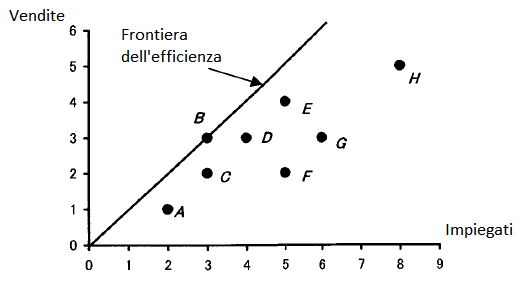
\includegraphics[scale=1]{Img/GraficoSISO.png}
\caption{Rappresentazione grafica dell'esempio}\label{FIG:SiSo}
\end{figure}

\paragraph{}Osserviamo dalla \autoref{FIG:SiSo} che per ogni negozio possiamo esprimere le vendite di ciascun dipendente come coefficiente angolare della retta che congiunge il punto del grafico corrispondente al negozio con l'origine. La retta con la pendenza maggiore (in questo caso quella passante per B) viene chiamata \emph{Frontiera dell'efficienza}. La scelta del nome \`e dovuta al fatto che i punti del grafico non posso trovarsi al di sopra di questa retta.

\paragraph{} Proseguiamo l'analisi dell'esempio valutando l'efficienza di tutti i negozi rispetto a B, con la formula
\begin{equation}\label{EQ:siso}
0\leq \dfrac{\text{Vendite per impiegato del negozio i-esimo}}{\text{Vendite per impiegato di B}} \leq 1
\end{equation}
ottenendo:
\begin{table}[H]
\centering
\begin{tabular}{lccccccccc}
\hline 
Negozio & A & B & C & D & E & F & G & H \\ 
\hline 
Efficienza & 0.5 & 1 & 0.667 & 0.75 & 0.8 & 0.4 & 0.5 & 0.625 \\ 
\hline 
\end{tabular}
\caption{Esempio con singolo input e singolo output} \label{TAB:SiSoContratta}
\end{table}

\paragraph{} A questo punto possiamo proporre delle strategia per rendere efficienti i negozi inefficienti: graficamente si traduce nell'avvicinare i punti rappresentanti i negozi alla frontiera dell'efficienza. Per esempio, il negozio A, pu\`o essere migliorato:
\begin{align}
&\text{riducendo l'input (numero di impiegati)}\label{EQ:input oriented}\\
&\text{aumentando l'output (vendite)}\label{EQ:output oriented}
\end{align}
Le due alternative proposte equivalgono rispettivamente ai punti $A_1$ e $A_2$ riportati in \autoref{FIG:SiSoNegozioA}: il punto $A_1$ corrisponde alla situazione in cui si riducono gli impiegati da 2 a 1, mantenendo le vendite inalterate; il punto $A_2$ invece, corrisponde ad un aumento delle vendite da 1 a 2 lasciando inalterato il numero di impiegati. Infine, tutti gli altri punti del segmento $\overline{A_1A_2}$ rappresentano un miglioramento del negozio A non ottenibile tramite le opzioni (\ref{EQ:input oriented}) o (\ref{EQ:output oriented}).

\begin{figure}[H]
\centering
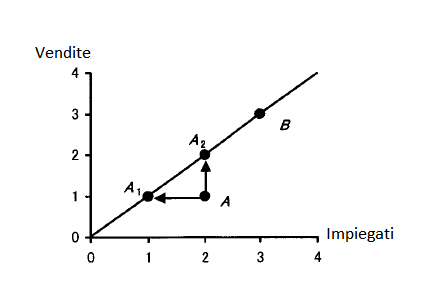
\includegraphics[scale=1]{Img/GraficoSiSoNegozioA.png}
\caption{Miglioramento del negozio A}\label{FIG:SiSoNegozioA}
\end{figure}

\begin{oss}
Il nome 'Data Envelopement Analysis' proviene dalla propriet\`a della frontiera dell'efficienza che avvolge (\emph{envelope}) tutte le rappresentazioni grafiche delle DMU.
\end{oss}
Non è ragionevole ritenere che la frontiera dell'efficienza si estenda all'infinito con la stessa pendenza. Analizzeremo questo problema in seguito utilizzando diversi modelli DEA. Tuttavia, diamo per scontato che questa linea è efficace nel range di interesse e chiamiamo tale assunzione 'rendimenti di scala costanti'.

\chapter{Metodi Test DEA} \label{CAP:due}
\section{CCR}
\bigskip

\paragraph{} Proseguiamo la trattazione esponendo il modello presentato per la prima volta da Charnes, Cooper e Rhodes nel 1978, che va sotto il nome di CCR.
\begin{definiz} Sia $\boldsymbol{X} \in \mathbb{R}^{m \times n}$ la matrice degli Input e sia $\boldsymbol{Y} \in \mathbb{R}^{s \times n}$  la matrice degli Output. Definiamo il CCR-Model nel seguente modo:
\begin{equation} \label{EQ:ccr-feq}
\begin{split}
(FP_o) \qquad & \max_{\boldsymbol{u,v}} \theta = \frac{u_1y_{1o} + \dots + u_sy_{so}}{v_1x_{1o} + \dots + v_mx_{mo}} \\
\text{t.c} \qquad & \frac{u_1y_{1j} + \dots + u_sy_{sj}}{v_1x_{1j} + \dots + v_mx_{mj}} \geq 1 \qquad (j=1,\dots,n)\\
& v_1,\dots,v_m \geq 0 \\
& u_1,\dots,u_s \geq 0 \\
\end{split}
\end{equation}
dove $v_j$ e $u_j$ rappresentano i pesi che associamo a rispettivamente a ciascun input e output.
\end{definiz}
\paragraph{}
Osserviamo che la \ref{EQ:ccr-feq} rappresenta un problema frazionale, quindi per poterlo eseguire con un elaboratore \'e risulta necessario riformularlo in modo da ottenere un problema lineare. 
\begin{definiz}
 Sia $\boldsymbol{X} \in \mathbb{R}^{m \times n}$ la matrice degli Input e sia $\boldsymbol{Y} \in \mathbb{R}^{s \times n}$  la matrice degli Output. Definiamo il CCR-Model nel seguente modo:
\begin{equation} \label{EQ:ccr-leq}
\begin{split}
(FP_o) \qquad & \max_{\boldsymbol{\mu,\nu}} \theta = \mu_1y_{1o} + \dots + \mu_sy_{so} \\
\text{t.c} \qquad & \nu_1x_{1o} + \dots + \nu_mx_{mo} = 1\\
& \mu_1y_{1j} + \dots + \mu_sy_{sj} \leq  \nu_1x_{1j} + \dots + \nu_mx_{mj} \quad (j = 1, \dots, n) \\
& \nu_1,\dots,\nu_m \geq 0 \\
& \mu_1,\dots,\mu_s \geq 0 \\
\end{split}
\end{equation}
dove $\nu_j$ e $\mu_j$ rappresentano i pesi che associamo a rispettivamente a ciascun input e output.
\end{definiz}
\begin{teor}
La \ref{EQ:ccr-feq} \'e equivalente alla \ref{EQ:ccr-leq}
\end{teor}
\begin{teor}(Unit Invariant Theorem)
La soluzione ottimale della \ref{EQ:ccr-feq} e \ref{EQ:ccr-leq} che indicheremo con $\max \theta = \theta^*$ sono indipendeti dalle unit\'a di misura con cui sono espressi output e input a patto che per ogni \emph{DMU} essi siano valutati con la stessa unit\'a di misura.
\end{teor}
\begin{definiz} (CCR-Efficiency) La DMU \'e efficiente per il CCR-Model se $\theta^* = 1$ e $(\boldsymbol{v^*, u^*})$, con $\boldsymbol{v^* \geq 0}$ e $\boldsymbol{u^* \geq 0}$. Altrimenti la DMU \'e inefficiente.
\end{definiz} 
\begin{definiz} Sia $\boldsymbol{X} \in \mathbb{R}^{m \times n}$ la matrice degli Input e sia $\boldsymbol{Y} \in \mathbb{R}^{s \times n}$  la matrice degli Output. Definiamo il CCR-Duale nel seguente modo:
\begin{equation}
\begin{split}
(DLP_0) \qquad & \min_{\theta, \boldsymbol{\lambda}} \theta \\
\text{t.c} \qquad & \theta\boldsymbol{x_o} - \boldsymbol{X\lambda} \geq 0 \\
& \boldsymbol{Y\lambda} \geq \boldsymbol{y_o} \\
& \boldsymbol{\lambda} \geq 0
\end{split}
\end{equation}
dove $\boldsymbol{\lambda} \in \mathbb{R}^{n}$ rappresenta il vettore dei pesi.
\end{definiz}
\begin{definiz}
Definiamo i vettori degli input in eccesso e degli output carenti, indicati rispettivamente come $\boldsymbol{s^{-}}$ e $\boldsymbol{s^{+}}$, nel seguente modo:
\begin{equation}
\begin{split}
\boldsymbol{s^{-}} = \theta \boldsymbol{x_o} - \boldsymbol{X \lambda} \text{ , }
\boldsymbol{s^{+}} = \boldsymbol{Y \lambda} -\boldsymbol{y_o}
\end{split}
\end{equation}
\end{definiz}
\begin{definiz} Usando la soluzione ottima del modello CCR-DUAL risolviamo il seguente sistema:
\begin{equation} \label{EQ:ccr-leq2}
\begin{split}
max_{\boldsymbol{\lambda, s^{-},s^{+}}} & \qquad \omega = \boldsymbol{es^{-} + es^{+}} \\ \text{t.c.} & \qquad \boldsymbol{s^{-}} = \theta^{*}\boldsymbol{x_o - X\lambda} \\ & \qquad
\boldsymbol{s^{+}} = \boldsymbol{Y\lambda - y_o} \\ & \qquad \boldsymbol{\lambda \geq 0 \text{ , } s^{-} \geq 0 \text{ , } s^{+} \geq 0} 
\end{split}
\end{equation}
dove $\boldsymbol{e} = (1,\ldots ,1)$. Definiamo tale modello II fase.
\end{definiz}
\begin{definiz}
Una soluzione ottima $(\boldsymbol{\lambda^*, s^{-*}, s^{+*}})$ del modello precedentemente esposto \'e  chiamata "max-slack solution". Se tale soluzione soddisfa $\boldsymbol{s^{-*} = 0}$ e $\boldsymbol{s^{+*} = 0}$ viene chiamata "zero-slack".
\end{definiz}
\begin{definiz}
Se una soluzione ottimale $(\boldsymbol{\theta^{*},\lambda^*, s^{-*}, s^{+*}})$ dei due modelli esposti soddisfa $\theta^* = 1$ ed \'e una soluzione zero-slack allora la DMU \'e chiamata CCR-efficient. Altrimenti \'e inefficiente.
\end{definiz}
\begin{oss}
Anche in questo caso possiamo definire i vettori di slack:
\begin{equation}
X\boldsymbol{\lambda + s^{-}} = \boldsymbol{x_o} \\
Y\boldsymbol{\lambda - s^{+}} = \theta\boldsymbol{y_o} 
\end{equation}
\end{oss}
\begin{definiz} (Pareto-Koopmans Efficiency) Una DMU \'e pienamente efficiente se e solo se non \'e possibile aumentare qualunque input o output senza peggiorarne un altro.
\end{definiz} 
\begin{teor} LE due definizioni di CCR-Efficient sono equivalenti.
\end{teor}
\begin{oss} Per una $DMU_{o}$ inefficiente, noi definiamo l'insieme di riferimento $E_{o}$, usando la max-slack solution ottenuta usando la \ref{EQ:ccr-leq2} e la \ref{EQ:ccr-leq}:
\begin{equation} \label{eq:insieme riferimento}
E_{o} = \lbrace j| \lambda_{j}^* \geq 0\rbrace \qquad (j\in \lbrace1, \dots, n\rbrace).
\end{equation}
Una soluzione ottimale pu\'o essere espressa come:
\begin{equation}
\begin{split}
\theta^*\boldsymbol{x_{o}} = & \sum_{j \in E_{o}} \boldsymbol{x_{j}\lambda^*_{j} + s^{-*}} \\
\boldsymbol{y_{o}} = & \sum_{j \in E_{o}} \boldsymbol{y_{j}\lambda^*_{j} - s^{+*}}
\end{split}
\end{equation}
Questo pu\'o essere interpretato come segue:
\begin{equation}
\boldsymbol{x_{o}} \geq \theta^* \boldsymbol{x_{o} - s^{-*}} = \sum_{j \in E_{o}} \boldsymbol{x_{j}\lambda^*_{j}}
\end{equation}
quindi
\begin{equation}
\boldsymbol{x_0} \geq \text{tecnice - mista inefficiente} \\
= \text{ una combinazione positiva degli input valutati}
\end{equation}
In modo analogo 
\begin{equation}
\boldsymbol{y_{o}} \leq \boldsymbol{y_{o} + s^{+*}} = \sum_{j \in E_{o}} \boldsymbol{y_{j}\lambda^*_{j}}
\end{equation}
quindi
\begin{equation}
\boldsymbol{y_0} \leq \text{output + carenze} \\
= \text{ una combinazione positiva degli output valutati}
\end{equation}
Concludendo queste relazioni suggeriscono che l'efficienza $(\boldsymbol{x_{o}, y_{o}})$ per una DMU pu\'o essere migliorata riducendo radialmente gli input usando la $\theta^*$ e eliminando gli eccessi $s^{-*}$. In modo analogo si pu\'o agire sugli output aumentando gli output della quantit\'a espressa da $s^{+*}$.
\end{oss}
\paragraph{} Dalle considerazioni fatte fino  ad ora possiamo enunziare la seguente definizione
\begin{definiz} Definiamo le \emph{CCR-projection} come:
\begin{equation} \label{EQ:project-crr-x}
\begin{split} 
\boldsymbol{\hat{x}_{o}} & = \boldsymbol{x_o - \Delta x_{o}} = \theta^*\boldsymbol{x_o - s^{-*}} \leq \boldsymbol{x_o}
\end{split}
\end{equation}
\begin{equation} \label{EQ:project-crr-y}
\begin{split}
\boldsymbol{\hat{y}_{o}} & = \boldsymbol{y_o + \Delta y_{o}} = \theta^*\boldsymbol{y_o + s^{+*}} \geq \boldsymbol{y_o} 
\end{split}
\end{equation}
\end{definiz}
\begin{teor}
Le migliorie $(\boldsymbol{\hat{x}_{o},\hat{y}_{o}})$ espresse dalle \ref{EQ:project-crr-x} e \ref{EQ:project-crr-y} sono CCR-efficient
\end{teor}
\begin{cor} I punti con coordinate $(\boldsymbol{\hat{x}_{o},\hat{y}_{o}})$ definite dalle \ref{EQ:project-crr-x} e \ref{EQ:project-crr-y} rappresentano il punto della frontiera dell'efficienza usata per valutare la performance della $DMU_{o}$.
\end{cor}
\begin{lemma}
Per il punto $(\boldsymbol{\hat{x}_{o},\hat{y}_{o}})$, esiste una soluzione ottima $(\boldsymbol{\hat{v}_{o},\hat{u}_{o}})$ per il problema $(LP_{e})$, la quale \'e duale a $(DLP_{e})$, tale che:
\begin{equation}
\begin{split}
\boldsymbol{\hat{v}_{o} \geq 0} & \\
\boldsymbol{\hat{u}_{o} \geq 0} & \\
\boldsymbol{\hat{v}_{o}x_{j} = \hat{u}_{o}y_{j}} & \quad (j \in E_{o}) \\
\boldsymbol{\hat{v}_{o}X \geq \hat{u}_{o}Y} & 
\end{split}
\end{equation}
\end{lemma}
\begin{teor} Le DMU in $E_{o}$ definito in \ref{eq:insieme riferimento} sono CCR-efficient
\end{teor}
\begin{teor} Ciascuna combinazione semipositiva delle DMU in $E_{o}$ \'e CCR-efficient.
\end{teor}
\begin{definiz}
Sia $\boldsymbol{X} \in \mathbb{R}^{m \times n}$ la matrice degli Input e sia $\boldsymbol{Y} \in \mathbb{R}^{s \times n}$  la matrice degli Output. Definiamo il CCR-Model orientato agli Output nel seguente modo:
\begin{equation} \label{eq1}
\begin{split}
(DLPO_0) \qquad & \min_{\theta, \boldsymbol{\lambda}} \theta \\
\text{t.c} \qquad & \boldsymbol{x_o} - \boldsymbol{X\lambda} \geq 0 \\
& \boldsymbol{Y\lambda} \geq \theta\boldsymbol{y_o} \\
& \boldsymbol{\lambda} \geq 0
\end{split}
\end{equation}
\end{definiz}
\begin{oss} Supponiamo di avere $(\theta^{*}, \boldsymbol{s^{*-}}, \boldsymbol{s^{*+}})$ soluzioni ottimali del CCR-Model e $(\mu^{*}, \boldsymbol{t^{*-}}, \boldsymbol{t^{*+}})$ soluzioni del CCR-Model orientato agli output, allora si ha che:
\begin{equation}
\boldsymbol{t^{*-}} = \boldsymbol{s^{*-}} / \theta^{*}, 
\boldsymbol{t^{*+}} = \boldsymbol{s^{*+}} / \theta^{*}
\end{equation}
\end{oss}
\section{BCC}
\bigskip
\begin{definiz}
Sia $\boldsymbol{X} \in \mathbb{R}^{m \times n}$ la matrice degli Input e sia $\boldsymbol{Y} \in \mathbb{R}^{s \times n}$  la matrice degli Output. Definiamo il BCC-Model nel seguente modo:
\begin{equation}
\begin{split}
(BCC_0) \qquad & \min_{\theta, \boldsymbol{\lambda}} \theta \\
\text{t.c} \qquad & \theta\boldsymbol{x_o} - \boldsymbol{X\lambda} \geq 0 \\
& \boldsymbol{Y\lambda} \geq \boldsymbol{y_o} \\
& \boldsymbol{\lambda} \geq 0 \\
& \boldsymbol{e\lambda} = 1
\end{split}
\end{equation}
dove $\boldsymbol{\lambda} \in \mathbb{R}^{n}$ rappresenta il vettore dei pesi ed $\boldsymbol{e} = (1 \dots 1)$.
\end{definiz}
\begin{definiz}
Se una soluzione ottima $(\theta^{*}, \boldsymbol{\lambda^{*}, s^{-*}, s^{+*}})$, ottenuta applicando la II fase al BCC-Model, soddisfa le condizioni $\theta^{*} = 1$ e "no slack solution" allora la DMU \'e chiamata BCC-efficient, altrimenti \'e inefficiente. 
\end{definiz}
\begin{definiz}
Per una $DMU_{o}$ inefficiente per BCC model definiamo il suo insieme di riferimento, $E_{o}$ basato su una soluzione ottima $\boldsymbol{\lambda^*}$ come:
\begin{equation} \label{eq: insieme riferimento BCC}
E_{o} = \lbrace j | \lambda_{j}^* \geq 0 \rbrace \quad (j \in \lbrace 1, \dots , n \rbrace
\end{equation}
\end{definiz}
\begin{definiz}
Definiamo le proiezioni del BCC-Model come:
\begin{equation} \label{eq:projection-bcc-x}
 \hat{\boldsymbol{x_{o}}} = \theta^* \boldsymbol{x_o - s^{-*}}
\end{equation}
\begin{equation}\label{eq:projection-bcc-y}
 \hat{\boldsymbol{y_{o}}} = boldsymbol{y_o + s^{+*}}
\end{equation}
\end{definiz}
\begin{teor}
Il punto di coordinate $(\boldsymbol{\hat{x_{o}}, \hat{y_{o}}})$ \'e BCC-efficient.
\end{teor}
\begin{teor}
Ogni DMU in $E_{o}$ associata a un $\lambda_{j}$ definita come \ref{eq: insieme riferimento BCC} \'e BCC-efficient
\end{teor}
\begin{teor}
Una DMU che ha un il valore minimo per ogni input, oppure che ha valore massimo per ciascun output, \'e BCC-efficient. 
\end{teor}
\begin{definiz}
Sia $\boldsymbol{X} \in \mathbb{R}^{m \times n}$ la matrice degli Input e sia $\boldsymbol{Y} \in \mathbb{R}^{s \times n}$  la matrice degli Output. Definiamo il BCC orientato all'Output nel seguente modo:
\begin{equation}
\begin{split}
(BCC_0-0) \qquad & \max_{\theta, \boldsymbol{\lambda}} \theta \\
\text{t.c} \qquad & \boldsymbol{X\lambda} \leq \boldsymbol{x_o} \\
& \boldsymbol{Y\lambda} \geq \theta\boldsymbol{y_o} \\
& \boldsymbol{\lambda} \geq 0 \\
& \boldsymbol{e\lambda} = 1
\end{split}
\end{equation}
dove $\boldsymbol{\lambda} \in \mathbb{R}^{n}$ rappresenta il vettore dei pesi ed $\boldsymbol{e} = (1 \dots 1)$.
\end{definiz}
\section{ADDITIVE MODEL}
\bigskip
\begin{definiz}
Sia $\boldsymbol{X} \in \mathbb{R}^{m \times n}$ la matrice degli Input e sia $\boldsymbol{Y} \in \mathbb{R}^{s \times n}$  la matrice degli Output. Definiamo l'ADDITIVE-MODEL nel seguente modo:
\begin{equation}
\begin{split}
(ADD_0) \qquad & \max_{\boldsymbol{\lambda, s^+, s^-}} \theta = \boldsymbol{es^- + e^+}\\
\text{t.c} \qquad & \boldsymbol{X\lambda + s^-} =  \boldsymbol{x_o} \\
& \boldsymbol{Y\lambda - s^+} = \boldsymbol{y_o} \\
& \boldsymbol{e\lambda} = 1 \\
& \boldsymbol{\lambda} \geq 0 , \boldsymbol{s^-} \geq 0 ,\boldsymbol{s^+} \geq 0 
\end{split}
\end{equation}
dove $\boldsymbol{\lambda} \in \mathbb{R}^{n}$ rappresenta il vettore dei pesi ed $\boldsymbol{e} = (1 \dots 1)$.
\end{definiz}
\begin{definiz}
Una DMU si dice \emph{ADD-efficient} se e solo se $\boldsymbol{s^{-*} = 0}$ e $\boldsymbol{s^{+*} = 0}$
\end{definiz}
\begin{teor} $DMU_{o}$ \'e ADD-efficient se e solo se \'e BCC-efficient
\end{teor}
\begin{teor} Definiamo $\hat{\boldsymbol{x_{o}}} = \boldsymbol{x_{o} - s^{-*}}$ e $\hat{\boldsymbol{y_{o}}} = \boldsymbol{y_{o} + s^{+*}}$. Allora il punto $(\hat{\boldsymbol{x_{o}}, \boldsymbol{y_{o}}}$ \'e ADD-efficient.
\end{teor}
\begin{definiz} Definiamo \emph{Mix} la proporzione nella quale gli input sono usati e gli output prodotti.
\end{definiz}
\begin{definiz} Dato un qualunque problema, una modello DEA \'e detto \emph{traslation invariant} se le traslazioni degli input e/o output iniziali generano un nuovo problema che ammette le stesse soluzioni del problema originale.
\end{definiz}
\begin{teor} L'Additive-model \'e \emph{traslation invariant}.
\end{teor}
\section{SBM MODEL}
\bigskip
\begin{definiz}
Sia $\boldsymbol{X} \in \mathbb{R}^{m \times n}$ la matrice degli Input e sia $\boldsymbol{Y} \in \mathbb{R}^{s \times n}$  la matrice degli Output. Definiamo SBM-DUALE nel seguente modo:
\begin{equation}
\begin{split}
(D-SBM) \qquad & \max_{\theta, \boldsymbol{v, u}} \theta \\
\text{t.c} \qquad & \theta + \boldsymbol{vx_o - uy_o} =  1 \\
& \boldsymbol{uY - vX} \leq \boldsymbol{0} \\
& \boldsymbol{v} \geq 1/m[1/\boldsymbol{x_o}] \\
& \boldsymbol{u} \geq \theta/s[1/\boldsymbol{y_o}] \\
\end{split}
\end{equation}
dove con $[1/\boldsymbol{x}]$ rappresenta il vettore $(1/x_1, \dots , 1/x_m)$.
\end{definiz}
\begin{definiz}
Una DMU si dice \emph{SBM-efficient} se e solo se $\theta = 1$
\end{definiz}
\begin{definiz} L'insieme degli indici corrispondenti ai valori positivi di $\lambda^*_{j}$ \'e chiamato insieme di riferimento per il punto $(\boldsymbol{x_{o}, y_{o}})$
\end{definiz}
\begin{teor} La soluzione ottima del SBM-Model \'e sempre minore o uguale a quella del CCR-model.
\end{teor}
\begin{teor} Una DMU \'e CCR-efficient se e solo se \'e SBM-efficient.
\end{teor}
\section{HYBRID}
\bigskip
Ci sono due tipo di approcci nella DEA: \emph{radiale} e \emph{non radiale}. La differenza esiste nella caratterizzazione degli input o degli output. Supponiamo di avere 4 input $(x_{1},x_{2},x_{3},x_{4})$ tali che $x_{1}, x_{2}$ sono radiali e gli altri no. Questa differenza potrebbe riflettersi sulla valutazione dell'efficienza. Nei modelli fino ad ora analizzati osserviamo che il CCR e il BCC hanno un approccio radiale mentre SBM ha un approccio non-radiale. In questa sezione mostreremo un approccio ibrido per misurare l'efficienza.
\begin{definiz} Sia $\boldsymbol{X} \in \mathbb{R}^{m \times n}$ la matrice degli Input e sia $\boldsymbol{Y} \in \mathbb{R}^{s \times n}$  la matrice degli Output. Decomponiamo la matrice degli input nella sua parte radiale $\boldsymbol{X^R} \in \mathbb{R}^{m_{1} \times n}$ e non radiale $\boldsymbol{X^{NR}} \in \mathbb{R}^{m_{2} \times n}$, con $m_{1} + m_{2} = m$. In modo del tutto analogo decomponiamo la matrice degli output in $\boldsymbol{Y^R} \in \mathbb{R}^{s_{1} \times n}$ e $\boldsymbol{Y^{NR}} \in \mathbb{R}^{s_{2} \times n}$, con $s_{1} + s_{2} = s$. Supponiamo infine che l'insieme dei dati considerati sia assolutamente positivo, allora definiamo l'insieme delle possibilit\'a produttive come:
\begin{equation}
P = \lbrace (\boldsymbol{x,y}) | \boldsymbol{x \geq X\lambda, y \leq Y\lambda , \lambda \geq 0 }\rbrace
\end{equation}
dove $\lambda \in \mathbb{R}^n$ \'e un vettore non negativo.
\end{definiz}
\begin{oss}
Diamo un equazione per descrivere un determinata $DMU(\boldsymbol{x_{o}, y_{o}) = (x_{o}^R, x_{o}^{NR}, y_{o}^R y_{o}^{NR}} \in P$ :
\begin{equation} \label{EQ:hybrid}
\begin{split}
\theta\boldsymbol{x_{o}^R} = & \boldsymbol{X^R\lambda + s^{R-}}\\
\boldsymbol{x_{o}^{NR}} = & \boldsymbol{X^{NR}\lambda + s^{NR-}}\\
\phi\boldsymbol{y_{o}^R} = & \boldsymbol{Y^R\lambda - s^{R+}}\\
\boldsymbol{y_{o}^{NR}} = & \boldsymbol{Y^{NR}\lambda - s^{NR+}}\\
\end{split}
\end{equation}
con $\theta \leq 1, \phi \geq 1, \boldsymbol{\lambda \geq 0, s^{R-} \geq 0, s^{NR-} \geq 0, s^{R+} \geq 0, s^{NR+} \geq 0}$.
Infine definiamo l'indice $\rho$ come:
\begin{equation}
\rho = \frac{1 - \frac{m_{1}}{m}(1 - \theta) - \frac{1}{m}\Sigma^{m_{2}}_{i=1} s^{NR-}_{i} / x_{io}^{NR}}{1 + \frac{s_{1}}{s}(\phi - 1) - \frac{1}{s}\Sigma^{s_{2}}_{r=1} s^{NR+}_{r} / y_{ro}^{NR}}
\end{equation}
\end{oss}
\begin{definiz}
La $DMU(\boldsymbol{x_{o},y_{o}})$ \'e hybrid efficient se e solo se $\rho = 1$ per ogni espressione possibile della \ref{EQ:hybrid}, cio\'e, $ \theta = 1, \phi = 1, \boldsymbol{s^{NR_{-}} = 0} , \boldsymbol{s^{NR_{-}} = 0}$  
\end{definiz}
\begin{definiz} Utilizzando le considerazioni fatte fino a questo punto possiamo definire il modello Hybrid nel seguente modo:
\begin{equation}
\begin{split}
\text{(HYBRID)} \qquad & \tau^* = \min t - \frac{m_1}{m}(\tau - \Theta) - \frac{1}{m} \Sigma^{m_2}_{i = 1} \frac{S^{NR_{-}}_{i}}{x^{NR}_{io}} \\
\text{t.c} \qquad & t + \frac{s_1}{s}(\Phi - t) + \frac{1}{s} \Sigma^{s_2}_{r = 1} \frac{S^{NR_{+}}_{r}}{y^{NR}_{ro}} \\
& \Theta\boldsymbol{x^{R}_o} \geq X^R \boldsymbol{\Lambda} \\
& t\boldsymbol{x^{NR}_o} = X^{NR}\boldsymbol{\Lambda} + S^{NR_{-}}\\
& \Phi\boldsymbol{y^{R}_o} \leq Y^R \boldsymbol{\Lambda} \\
& t\boldsymbol{y^{NR}_o} = Y^{NR}\boldsymbol{\Lambda} - S^{NR_{+}}\\
& \Theta \leq t, \Phi \geq t, \boldsymbol{\Lambda \geq 0}, \boldsymbol{S^{NR_{+}} \geq 0}, \boldsymbol{S^{NR_{-}} \geq 0}, 
\end{split}
\end{equation}
\end{definiz}
\begin{teor} La $DMU(\boldsymbol{x_o, y_o})$ \'e hybrid efficient se e solo se $\tau = 1$. 
\end{teor}
\begin{oss} Sia $(t^*, \Theta^*, \Phi^*, \boldsymbol{\Lambda^*, S^{NR_{-*}}, S^{NR_{+*}}})$ la soluzione ottima del HYBRID allora definiamo:
\begin{equation}
\begin{split}
\theta^* & = \frac{\Theta^*}{t^*} \\
\phi^* & = \frac{\Phi^*}{t^*} \\
\boldsymbol{\lambda}^* & = \frac{\boldsymbol{\Lambda}^*}{t^*} \\
\boldsymbol{s^{NR_{-*}}} & = \frac{\boldsymbol{S^{NR_{-*}}}}{t^*} \\
\boldsymbol{s^{NR_{+*}}} & = \frac{\boldsymbol{S^{NR_{+*}}}}{t^*} \\
\end{split}
\end{equation}
Se $\tau \leq 1$ allora definiamo le proiezioni del HYBRID model come:
\begin{equation}
\begin{split}
\boldsymbol{\hat{x}_o^R} & \longleftarrow \theta^* \boldsymbol{x_o^R} \\
\boldsymbol{\hat{x}_o^{NR}} & \longleftarrow \boldsymbol{x_o^{NR}} - \boldsymbol{s}^{NR_{-*}}\\
\boldsymbol{\hat{y}_o^R} & \longleftarrow \phi^* \boldsymbol{y_o^R} \\
\boldsymbol{\hat{y}_o^{NR}} & \longleftarrow \boldsymbol{y_o^{NR}} + \boldsymbol{s}^{NR_{+*}}\\
\end{split}
\end{equation}
\end{oss}
\begin{teor} Le proiezioni definite nell'osservazione precedente sono \emph{hybrid efficient}.
\end{teor}


\chapter{Ritorno di Scala} \label{CAP:tre}
\section{Ritorno di scala}
\bigskip

TODO: scrivere l'introduzione
Ora consideriamo le condizioni per i ritorni di scala dei seguenti modelli

\section{Il ritorno di scale del BBC-Model}

Consideriamo le equazioni del BCC model:
\begin{equation}
\begin{split}
\max \qquad & z = \boldsymbol{uy_o} - u_o \\
\text{t.c} \qquad & \boldsymbol{vx_o = 1} \\
& \boldsymbol{-vX + uY -} u_o\boldsymbol{e \leq 0} \\
& \boldsymbol{v \geq 0, u \geq 0,} u_o \text{ qualunque} \\ 
\end{split}
\end{equation}
possiamo esprime i ritorni di scala per tale modello utilizzando il seguente teorema.

\begin{teor} Assumiamo che $(\boldsymbol{x_o, y_o})$ sia una punto della frontiera dell'efficienza allora abbiamo che: \\
(i)L'Increasing returns-to-scale prevale su $(\boldsymbol{x_o, y_o})$ se e solo se $u^*_o < 0$ per ogni soluzioni ottimale. \\
(ii)Il Decreasing returns-to-scale prevale su $(\boldsymbol{x_o, y_o})$ se e solo se $u^*_o > 0$ per ogni soluzioni ottimale.\\
(ii)Il Constant returns-to-scale prevale su $(\boldsymbol{x_o, y_o})$ se e solo se $u^*_o = 0$ in alcune soluzioni ottimali.\\
\end{teor}

\section{Il ritorno di scale del CCR-Model}

\begin{teor}
Sia $(\boldsymbol{x_o, y_o})$ sia una punto della frontiera dell'efficienza, e consideriamo la soluzione ottima ottenuta dal CCR-Model $(\lambda^*_1, \dots, \lambda^*_n)$. Il ritorno di scale in tale punto può essere determinato dalle seguenti condizioni:\\
(i) Se $\Sigma^n_{j = 1} \lambda^*_j = 1$ in ciascuna soluzione ottimale allora prevale il constant returns-to-scale \\
(ii) Se $\Sigma^n_{j = 1} \lambda^*_j > 1$ in ciascuna soluzione ottimale allora prevale il decreasing returns-to-scale \\
(iii) Se $\Sigma^n_{j = 1} \lambda^*_j < 1$ in ciascuna soluzione ottimale allora prevale l'increasing returns-to-scale \\
\end{teor}

Enunciamo adesso un teorema che mette in relazione il BBC-Model e CCR-Model.

\begin{teor}
Consideriamo le soluzioni ottimali del CCR-Model e del BCC-Model si ha che: \\
(i) $u^*_o > 0$ per ogni soluzione ottimale del BBC-Model se e solo se $\Sigma^n_{j = 1} \hat{\lambda}^*_j > 1$ per ogni soluzione ottimale del CCR-Model corrispondente.\\
(ii) $u^*_o < 0$ per ogni soluzione ottimale del BBC-Model se e solo se $\Sigma^n_{j = 1} \hat{\lambda}^*_j < 1$ per ogni soluzione ottimale del CCR-Model corrispondente.\\
(iii) $u^*_o = 0$ per alcune soluzione ottimali del BBC-Model se e solo se $\Sigma^n_{j = 1} \hat{\lambda}^*_j = 1$ per alcune soluzioni ottimali del CCR-Model corrispondente.\\
\end{teor}

\section{Grandezze di scala produttive}

\begin{teor} Una $DMU_o$ efficiente per il CCR-Model sar\'a efficiente anche per il BCC-Model model e prevar\'a il constant returns-to-scale.
\end{teor}
TODO scrivere def MPSS
\begin{definiz}Una $DMU_o$ si dice MPSS se soddisfa le seguenti condizioni:
\begin{equation}
\begin{split}
\text{(i)} \qquad & \beta^* / \alpha^* \\
\text{(ii)} \qquad & \text{tutti gli slack sono zero}\\
\end{split}
\end{equation}
\end{definiz}
\begin{teor} Consideriamo una $DMU_o$ con input e output rappresentati dai vettori $\boldsymbol{x_o, y_o}$. Si ha che una condizione necessaria per essere MPSS \'e  $\beta^*/\alpha^* = \max \beta/\alpha = 1$. In tale caso $\beta^* = \alpha^*$ e i ritorni di scala sono costanti. 
\end{teor}
\begin{teor} Nel BCC model un insieme di riferimento per ciascuna $DMU$ non efficiente non può includere allo stesso tempo increasing e decreasing return-to-scale DMUs.
\end{teor}
\begin{cor} \label{cor:return-to-scale} 
Sia $E_o$ l'insieme di riferimento di una $DMU(\boldsymbol{x_o, y_0})$. Allora, $E_o4$ sar\'a costituita da una delle seguenti combinazioni di $DMU$ efficienti:
\begin{equation}
\begin{split}
\text{(i)} \qquad & \text{Tutte le DMU sono IRS} \\
\text{(ii)} \qquad & \text{Tutte le DMU sono CRS} \\
\text{(iii)} \qquad & \text{Tutte le DMU sono DRD} \\
\text{(iv)} \qquad & \text{le DMU sono IRS o CRS} \\
\text{(v)} \qquad & \text{le DMU sono DRS o CRS} \\
\end{split}
\end{equation}
dove IRS, CRS e DRS sta per increasing, constant e decresing return-to-scale rispettivamente.
\end{cor}
\begin{teor} \label{EQ:return-to-scale}
Sia $(\hat{\boldsymbol{x_o}}, \hat{\boldsymbol{y_o}})$ la proiezione efficiente di una $DMU_o$ che risulti BCC-inefficient, sia $E_o$ l'insieme di riferimento relativo alla $DMU_o$. Allora si ha che:\\\\
1. $(\boldsymbol{\hat{x_o}}, \hat{\boldsymbol{y_o}})$ \'e IRS se $E_o$ /'e costituito da $DMUs$ del tipo (i) o (iv) del Corollario \ref{cor:return-to-scale} \\\\
2. $(\boldsymbol{\hat{x_o}}, \hat{\boldsymbol{y_o}})$ \'e DRS se $E_o$ /'e costituito da $DMUs$ del tipo (iii) o (v) del Corollario \ref{cor:return-to-scale} \\\\
\end{teor}
\section{Rilassamento della condizione di convessit\'a}
\bigskip
Possiamo estendere il BCC model rilassando la condizione di convessit\'a $\boldsymbol{e\lambda} = 1$ utilizzando:
\begin{equation}
L \leq \boldsymbol{ e\lambda} \leq U
\end{equation}
dove $L (0 \leq L \leq 1)$ e $U (1 \leq U)$ sono rispettivamente upper e lower bound per la somma dei $\lambda_j$. Notiamo che la condizione $L = 0$ e $U = \infty$ corrisponde al CCR model.
\subsection{Increasing Returns-to-Scale (IRS) Model}
\bigskip
Il caso $L = 1, U = \infty$ \'e chiamato IRS o NDRS (Non decreasing Returns-to-Scale) model. In questo modello il vincolo imposto ai valori di $\boldsymbol{\lambda}$ \'e:
\begin{equation}
\boldsymbol{e\lambda \geq 1}
\end{equation}
Osserviamo che la condizione $L=1$ corrisponde al fatto che non sarà possibile ridurre i pesi della $DMU$ ma sar\'a possibile espandere quest'ultimi all'infinito (TODO inserire immagine con esempio).
\subsection{Decreasing Returns-to-Scale (DRS) Model}
\bigskip
Il caso $L = 0, U = 1$ \'e chiamato DRS o NIRS (Non increasing Returns-to-Scale) model. In questo modello il vincolo imposto ai valori di $\boldsymbol{\lambda}$ \'e:
\begin{equation}
0 \leq \boldsymbol{e\lambda} \leq 1
\end{equation}
Osserviamo che la condizione $U=1$ corrisponde al fatto che non sarà possibile aumentare i pesi della $DMU$ (TODO inserire immagine con esempio).
\subsection{Generalized Returns-to-Scale (DRS) Model}
\bigskip
Il caso $0 \leq L \leq 1, U \geq 1$ \'e chiamato Generalized Returns-to-Scale model. In questo modello \'e possibile definire dei valori di controllo per determinare dei range ammissibili in cui far variare i return-to-scale (TODO inserire immagine con esempio).
\section{Decomposizione dell'inefficienza tecnica}
\bigskip

Nello studio delle DEA ricopre una notevole importanza lo studio delle cause che creano l'inefficienza in una DMU.(TODO continuare l'intro)

\subsection{Scale efficiency}

\begin{definiz} \label{EQ:scale efficiency}
Consideriamo il risultato ottenuto dal CCR e BCC model di una DMU rispettivamente rappresentati da $\theta^*_{CCR}$ e $\theta^*_{BCC}$. La \emph{scale efficiency} \'e definita da
\begin{equation}
SE = \frac{\theta^*_{CCR}}{\theta^*_{BCC}}
\end{equation}
\end{definiz}



\chapter{Modelli con moltiplicatori limitati} \label{CAP:quattro}
\section{Ritorno di scala}
\bigskip



%\include{conclusioni}

%\include{ringraziamenti}

%\include{bibliografia}

\end{document}